\section{}
% A diving board is modeled as a beam of length 3𝐿 and is simply supported at 𝑥 = 0 and 𝑥 = 𝐿. 
% The diving board has a uniform density and cross-sectional area
\textit{A diving board is modeled as a beam of length $3L$ and is simply supported at $x = 0$ and $x = L$. The diving board has a uniform density and cross-sectional area $A$.}

\begin{figure}[H]
    \centering
    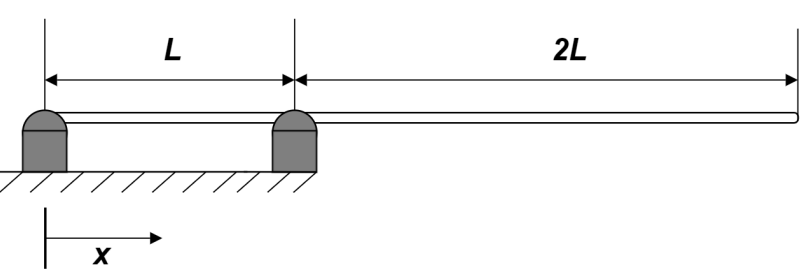
\includegraphics[width=0.6\linewidth]{Questions/Figures/Q5 Problem Statement a).png}
\end{figure}

\subsection{}
\textit{Estimate the lowest natural frequency of the beam in terms of $E$, $I$, $\rho$, $A$, $L$, using Rayleigh’s Quotient. Assume a mode shape of $\mathbb{Y}(x) = Lx - x^2$.}

Recall the Rayleigh's Quotient for continuous systems:
\begin{align*}
    p^2 &= \displaystyle\frac{\displaystyle \int_{0}^{3L} EI \left(\frac{d^2 \mathbb{Y}}{dx^2}\right)^2 dx + \sum_{i = 1}^{s} k_i \left(\mathbb{Y}(x_i)\right)^2}{\displaystyle \int_{0}^{3L} \rho A \left(\mathbb{Y}\right)^2 dx + \sum_{j = 1}^{n} m_j \left(\mathbb{Y}(x_j)\right)^2}
\end{align*}
Let us evaluate convenient quantities for the given beam:
\begin{align*}
    \frac{d^2 \mathbb{Y}}{dx^2} &= -2 \\
    \left(\frac{d^2 \mathbb{Y}}{dx^2}\right)^2 &= 4 \\
    \mathbb{Y}^2 &= (Lx - x^2)^2 = L^2 x^2 - 2Lx^3 + x^4
\end{align*}
Then the terms of the Rayleigh's Quotient become:
\begin{align*}
    \int_{0}^{3L} EI \left(\frac{d^2 \mathbb{Y}}{dx^2}\right)^2 dx &= 4 EI \int_{0}^{3L} dx \\
    &= 12 EI L \\
    \int_{0}^{3L} \rho A \left(\mathbb{Y}\right)^2 dx &= \rho A \int_{0}^{3L} L^2 x^2 - 2Lx^3 + x^4 dx \\
    &= \rho A \left[\frac{L^2 x^3}{3} - \frac{2L x^4}{4} + \frac{x^5}{5}\right]_{0}^{3L} \\
    &= \rho A \left[\frac{L^2 (3L)^3}{3} - \frac{2L (3L)^4}{4} + \frac{(3L)^5}{5}\right] \\
    &= \frac{171 \rho A L^5}{10} \\
\end{align*}
Therefore, the Rayleigh's Quotient for the given beam is:
\begin{align*}
    p^2 &= \frac{12 EI L}{\frac{171 \rho A L^5}{10}} \\
    &= \frac{120 EI}{171 \rho A L^4} \\
    &= \frac{40 EI}{57 \rho A L^4}
\end{align*}
And the lowest natural frequency is:
\begin{empheq}[box=\fbox]{align*}
    p &= \sqrt{\frac{40}{57}} \cdot \sqrt{\frac{EI}{\rho A L^4}}
\end{empheq}

\subsection{}
% (5 pts) Divers have complained that the board is too bouncy. A proposed solution is to 
% install a mass positioned as shown below to reduce the natural frequency to 90% of its 
% original value. If the mass of the diving board is 60 kg, determine the mass 𝑀 that must be 
% installed
\textit{Divers have complained that the board is too bouncy. A proposed solution is to install a mass positioned as shown below to reduce the natural frequency to 90\% of its original value. If the mass of the diving board is 60 kg, determine the mass $M$ that must be installed.}

The addition of the mass adds a term to the denominator of the Rayleigh's Quotient. The new term is 
\begin{align*}
    M \left(\mathbb{Y}(2L)\right)^2 &= M \left(L(2L) - (2L)^2\right)^2 \\
    &= 4M L^4
\end{align*}
The Rayleigh's Quotient for the system with the added mass is then
\begin{align*}
    p_2^2 &= \frac{12 EI L}{\frac{171 \rho A L^5}{10} + 4M L^4} 
\end{align*}
Since we want $p_2 = 0.9 p_1$, we have
\begin{verbatim}
syms M L A rho EI
p_1_sq = 40 * EI / (57 * rho * A * L^4);
p_2_sq = 12 * EI * L / ((171 * rho * A * L^5) / 10 + 4 * M * L^4);

simplify(p_2_sq / p_1_sq)
eqn = p_2_sq / p_1_sq == 0.9^2;
eqn = subs(eqn, A*L*rho, 20);
M = solve(eqn, M)

>> (171*A*L*rho)/(40*M + 171*A*L*rho)

>> M = 20.055555555555555555555555555556
\end{verbatim}
So,
\begin{align*}
    \frac{p_2^2}{p_1^2} &= 0.9^2 \\
    &= \frac{171 A L \rho}{40 M + 171 A L \rho} 
\end{align*}
Since the mass of the diving board is 60 kg, 
% $m = 3 A L \rho = 60$, so $A L \rho = 20$. Then,
\begin{align*}
    m &= 3 A L \rho = 60 \\
    \implies A L \rho &= 20
\end{align*}
Then,
\begin{align*}
    0.9^2 &= \frac{171 \cdot 20}{40 M + 171 \cdot 20} \\
    0.81 &= \frac{3420}{40 M + 3420} \\
    \implies \Aboxed{M &= 20.056 \text{ kg}}
\end{align*}